\subsection{Закон сохранения энергии и типы орбит}
Закон сохранения энергии. $E_0$ - константа, равна сумме кинетической и потенциальной энергии единичной массы.$$\frac{v^2}{2}-\frac{GM}{r}=E_0$$

Если $E_0>0$, то траектория тела --- гипербола, ветви которой асимптотически приближаются к двум прямым.

Если $E_0=0$, то траектория тела --- гипербола. При параболической и гиперболический траекториях движение не ограничено.

Если $E_0<0$, то траектория тела --- эллипс. При эллиптической траектории движение ограничено.

Параболическая скорость - минимальная скорость, при которорй тело покидает центральную массу$M$.$$V_p=\sqrt{\frac{2GM}{r}}$$

На рис. 1 представлены примеры возможных траекторий тела относительно центрального (точка C).

При $v_0>v_p$ (пароболическая скорость) --- тело движется по гиперболе,при $v_0=v_p$ --- тело движется по пораболе, а при $v_0<v_p$ --- по эллипсу.
\begin{center}
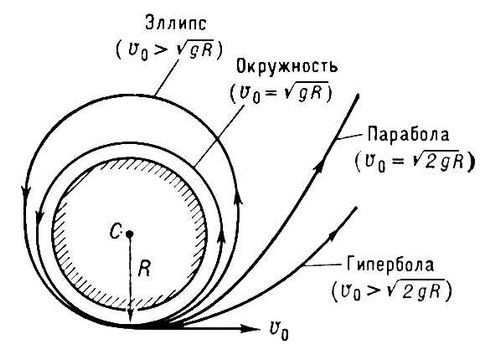
\includegraphics[scale=0.35]{Space-speed}
\begin{figure}[h!]
\caption{ Возможные траектории тела}
\end{figure}
\end{center}